\subsection{XRCE-DDS Layer APIs}
% - NOTE: -------------------------------------------------------------
\subsubsection{session.c}

\textbf{1. \apiarg{uxr\_run\_session\_until\_data}{uxrSession* session, int timeout\_ms}}: Keeps communication between the Client and the Agent. This function involves the following actions:
\begin{itemize}
    \item [(1)] flushing all the output streams sending the data through the transport (e.g., UCP, UART\dots). This actions will be performed in a loop until a data message is received or the \str{timeout} is exceeded.
    \item [(2)] listening messages from the Agent calling the associated callback (topic, status, request and replies).
\end{itemize}

\begin{figure}[htbp!]
    \centering
    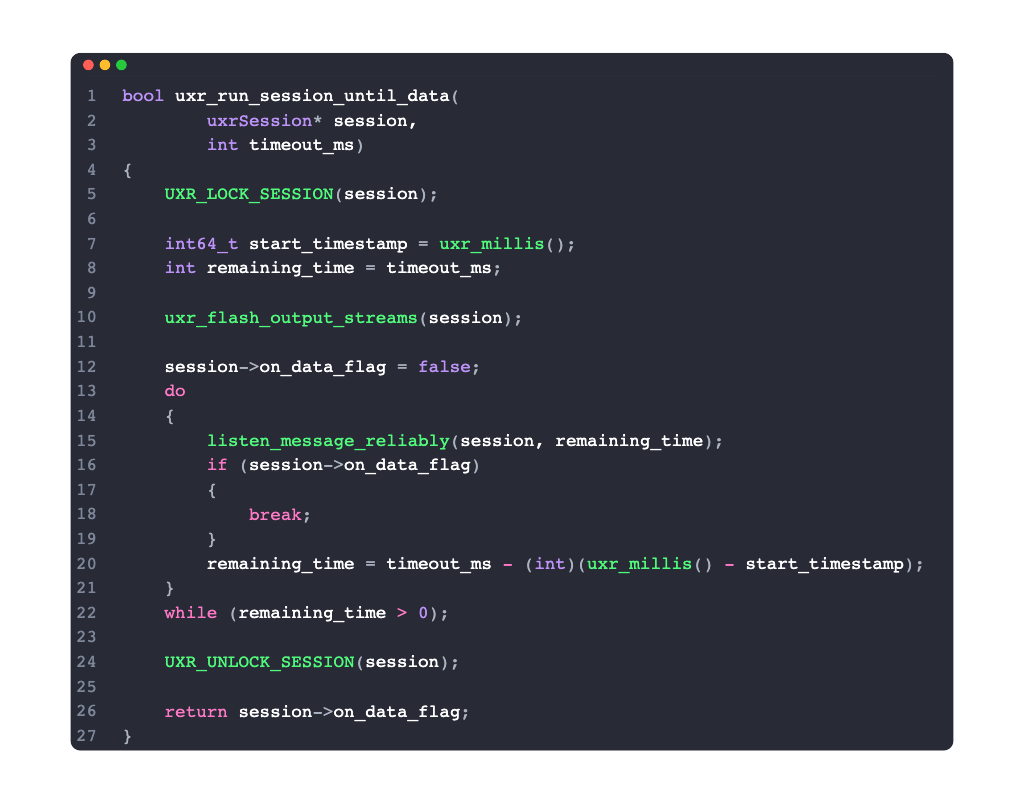
\includegraphics[width=1\linewidth]{Sec/Implementation/uxr/fig/uxr_run_session_until_data.png}
    \caption{Function code: uxr\_run\_session\_until\_data()}
    \vspace{-0.1in}
\end{figure}

As can be seen in function \api{uxr\_run\_session\_until\_data~()}, it first calls \apiarg{UXR\_LOCK\_SESSION}{session}, which finally invokes \apiarg{xSemaphoreTakeRecursive}{mutex->impl, portMAX\_DELAY} on FreeRTOS, or \apiarg{pthread\_mutex\_lock}{\&mutex->impl} on POSIX platform.

\textbf{2. \apiarg{uxr\_stream\_id}{uxrSession* session, int timeout\_ms}}:
\todo{HERE!!!!!!!!!!!!!!!!!!}

\textbf{3. \apiarg{uxr\_prepare\_best\_effort\_buffer\_to\_send}{uxrSession* session, int timeout\_ms}}:

\textbf{4. \apiarg{uxr\_stamp\_session\_header}{uxrSession* session, int timeout\_ms}}: